\chapter{Edge Detection}

\section{What is an Edge?}

"边缘"是图像中的一个区域,在这个区域中,沿着图像的一个方向,
像素强度值 (或者说对比度) 发生了"显著"的变化,而在其正交方向上,
像素强度值 (或对比度) 几乎没有变化.

\begin{figure}[htbp]
    \centering
	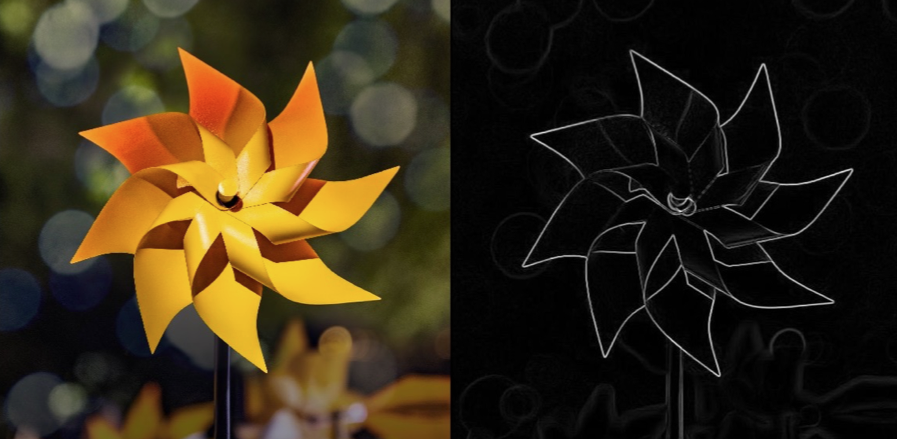
\includegraphics[scale=0.2]{figures/edge.png}
	\caption{边缘检测示意图}
\end{figure}

"边缘" 不等于 "梯度大的区域". 因为也有可能是噪声(多方向都梯度大).

\section{Criteria for Optimal Edge Detection}

\begin{equation}
\text{Accuracy}=\frac{\text{TP}+\text{TN}}{\text{TP}+\text{FP}+\text{TN}+\text{FN}} = \frac{\text{所有检测出的边缘}}{\text{所有边缘}}
\end{equation}

\begin{equation}
\text{Precision}=\frac{\text{TP}}{\text{TP}+\text{FP}} = \frac{\text{正确检测的边缘}}{\text{所有检测出的边缘}}
\end{equation}

\begin{equation}
\text{Recall}=\frac{\text{TP}}{\text{TP}+\text{FN}} = \frac{\text{正确检测的边缘}}{\text{所有真正的边缘}}
\end{equation}

\begin{itemize}
    \item TP: true positives, 正确检测的边缘
    \item FP: false positives, 错误检测的边缘
    \item TN: true negatives, 正确未检测的边缘
    \item FN: false negatives, 错误未检测的边缘
\end{itemize}

Precision 和 Recall 都代表着你检测出的真正边缘所占比例,但是 Precision 的分母
是你检测出的边缘,Recall 的分母是真正的边缘. 最好是同时有高的 Precision 和 Recall.

\vspace{1em}

我们还需要选择什么是 True:

\begin{itemize}
    \item Good Localization: 边缘应该在真实边缘的附近,而不是在其他地方. 通过设置阈值 $\epsilon$ 来控制.
    \item Single response constraint: 一个边缘应该只被检测一次. 抑制冗余的边缘.
\end{itemize}

\section{Non-Maximal Suppression (NMS)}

非最大值抑制,顾名思义,就是抑制非最大值,这里的最大值指的是梯度的局部最大值.

在计算出了所有点的梯度之后,会有很多像素的梯度大于设定的阈值,而我们希望最后得出的边缘像素真的看起来
像一条线而不是一块区域,所以 NMS 的目的是为了抑制那些不是边缘的像素,只保留那些是边缘的像素.

\begin{figure}[htbp]
    \centering
	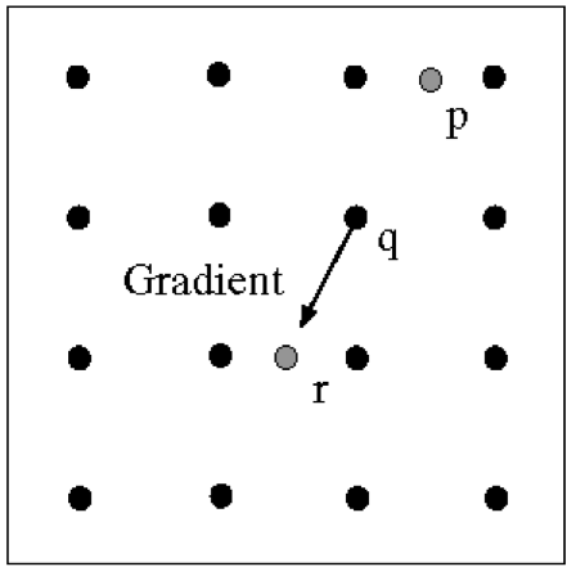
\includegraphics[scale=0.2]{figures/NMS.png}
	\caption{NMS示意图}
\end{figure}

对于一个边缘像素的候选点,我们认为它是边缘当:它比它梯度方向的两个点 $q+\nabla q$ 和 $q-\nabla q$ 的梯度值大,
也就是这个点的梯度大小是局部最大值的时候.

为什么这样可以?一个不严谨但通俗的解释是:我们考虑什么时候需要 NMS,当一个边宽度大于 1 个像素的时候,比如这个线是 4 像素宽,那么
我们沿着这个线的垂直方向(也即梯度方向)看,只找一个梯度变化最大的点,其他点丢掉,就能实现 NMS 的效果。

\begin{figure}[htbp]
    \centering
	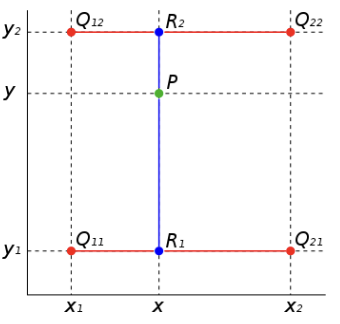
\includegraphics[scale=0.4]{figures/bilinear.png}
	\caption{双线性插值}
\end{figure}

\[
\begin{aligned}
    &R_{1}{:}\quad f(x,y_{1})=\frac{x_{2}-x}{x_{2}-x_{1}}f(Q_{11})+\frac{x-x_{1}}{x_{2}-x_{1}}f(Q_{21}),\\
    &R_{2}{:}\quad f(x,y_{2})=\frac{x_{2}-x}{x_{2}-x_{1}}f(Q_{12})+\frac{x-x_{1}}{x_{2}-x_{1}}f(Q_{22}).\\
    &P{:}\quad f(x,y)=\frac{y_{2}-y}{y_{2}-y_{1}}f(x,y_{1})+\frac{y-y_{1}}{y_{2}-y_{1}}f(x,y_{2})\\&=\frac{y_{2}-y}{y_{2}-y_{1}}\left(\frac{x_{2}-x}{x_{2}-x_{1}}f(Q_{11})+\frac{x-x_{1}}{x_{2}-x_{1}}f(Q_{21})\right)+\frac{y-y_{1}}{y_{2}-y_{1}}\left(\frac{x_{2}-x}{x_{2}-x_{1}}f(Q_{12})+\frac{x-x_{1}}{x_{2}-x_{1}}f(Q_{22})\right)
\end{aligned}
\]

计算这个点梯度方向的点的梯度值可以使用双线性插值法(先插出 $R_1$ 和 $R_2$,然后再插出 $P$),也即把这个点周围的四个点的梯度按照横纵距离反比加权(即离这个点越近,最后的加权就越大).

当然,NMS 是一个思想而不是针对边缘检测的算法,比如对于 keypoint detection,object detection (like YOLO) 都可以使用 NMS,
实现的思路都很类似,使用一个打分函数看这个备选点 (bounding box) 是不是比跟它相邻 (冲突) 的点 (bounding box) 好,如果是就保留,否则就抑制.

\section{A Simplified Version of NMS}

\begin{figure}[htbp]
    \centering
	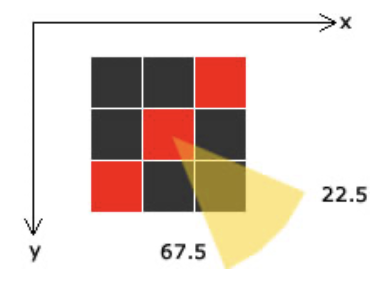
\includegraphics[scale=0.55]{figures/simple_NMS.png}
	\caption{简化版本的双线性插值}
\end{figure}

一个 NMS 的简化版本是把双线性插值省去,直接让这个像素的梯度大于它梯度方向的那两个相邻像素的梯度. 这利用了图片的离散化,因为这个像素只可能和周围 8 个像素竞争 NMS 当边缘.

\begin{figure}[htbp]
    \centering
	
\includegraphics[scale=0.55]{figures/simple_NMS_2.png}
	\caption{简化版本的双线性插值颜色分组}
\end{figure}

\section{Hysteresis Thresholding}

考虑如何连接起来被通过 NMS 的 edge 连成一条 edge(edge linking).

\textbf{写作业的时候千万注意这里的 $y$ 轴是竖直向下的, 不要搞反了.}

这里有一个 trick,使用高阈值 (maxVal) 开始边缘曲线,只要 edge 没有低于 minVal,就继续.而一旦低于 minVal,就停止.

\begin{itemize}
    \item 像素梯度值大于 maxVal 的应该保留.
    \item 像素梯度值小于 minVal 的应该被抑制.
\end{itemize}

如何决定 maxVal 和 minVal?

\begin{itemize}
    \item maxVal = 0.3 $\times$ 通过 NMS 的像素的平均梯度值
    \item minVal = 0.1 $\times$ 通过 NMS 的像素的平均梯度值
\end{itemize}

其中系数是可调参数.

\section{The trade-off of Gaussian filtering}

$\sigma$ 是高斯滤波的标准差参数,决定了平滑的程度。在 Canny 边缘检测中,高斯滤波用于降低图像中的噪声,但也会影响边缘的清晰程度。

\begin{itemize}
    \item 较小的 $\sigma$ 值(如 $\sigma = 1$)表示较少的平滑,保留了更多的细节和边缘,但可能会对噪声更加敏感。考虑极端情况 $\sigma = 0$,此时完全没有平滑(因为此时高斯函数退化为狄拉克函数),噪声会完全保留,导致边缘检测效果不佳。
    \item 较大的 $\sigma$ 值(如 $\sigma = 2$)表示更强的平滑,能够更好地去除噪声,但会使边缘变得模糊,定位不够精确。
\end{itemize}

因此,$\sigma$ 体现了 \textbf{平滑与边缘定位之间的权衡}:增大 $\sigma$ 可以减少噪声的影响,但会导致边缘检测的精确度下降。

\begin{figure}[htbp]
    \centering
	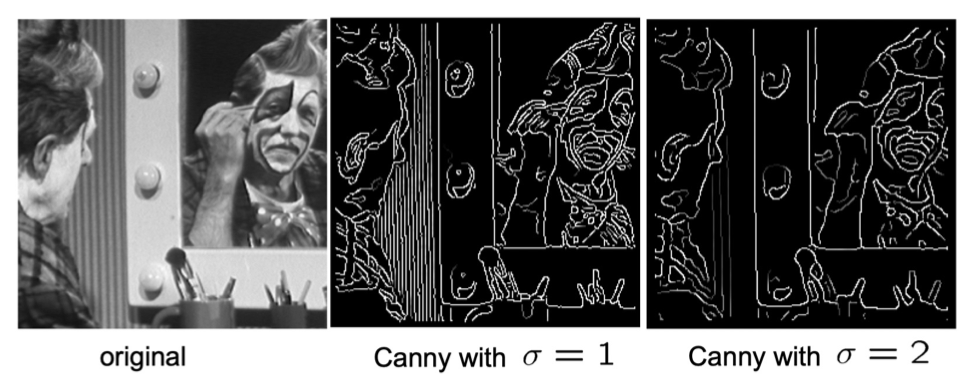
\includegraphics[scale=0.2]{figures/tradeoff-in-gauss-filtering.png}
	\caption{高斯滤波的权衡}
\end{figure}

